\end{multicols*}

\mysection{Effects}{game-effects}

Most effects have a \Duration attached to them, as defined in the rules (or by the Arbiter). Effects on Monsters can sometimes differ from Effects on Adventurers, and are detailed where appropriate.

\myimage{game/EffectDivider}

\begin{multicols*}{2}


  \mysubsection{Addicted}{effect-addicted}

  See more info on \mylink{Addiction}{gear-narcotics-addiction} in the section on \mylink{Narcotics}{gear-narcotics} under \mylink{Gear}{gear}.

  \mysubsection{Afraid}{effect-afraid}

  If you are Afraid of something, you must make an \mylink{Insanity}{adventurer-kismet-insanity} try when you approach or attack the object of your fear. If you damage the object of your Fear, the Fear is immediately dispelled.

  \mybold{Effect on Monsters:} If a Monster is Afraid of something, it will try to run away.  If left to its own devices, it will hide in the adjacent room / area that is most safe and return when the duration is up.  Monsters resist Fear with a morale check.

  \mysubsection{Anathema}{effect-anathema}

  You cannot benefit from magical healing or be the target of helpful magic (note: \mylink{Leechcraft}{arcana-leechcraft} isn't magical healing).  You automatically fail any \SAVE{Hexes}, and you cannot gain Glory through Carousing.

  \mybold{Effect on Monsters:} The Monster cannot regenerate; Save tries are made at a -4.

  \mysubsection{Befuddled}{effect-befuddled}

  If you are Befuddled, you cannot tell any two creatures apart - everyone looks the same. Whenever you attack, you attack a random creature.  When you cast a spell, you cast a random spell at a target picked randomly from all eligible ones.  Whenever you try to run through a door, you run through a random door.  The Arbiter should feel free to dictate additional effects as necessary.

  \mysubsection{Bleeding}{effect-bleeding}

  If you are Bleeding, you lose 1 Flesh at the Top of every Moment.  This doesn't stack (i.e. you can't Bleed for 2 damage every Moment).

  \mysubsection{Blinded}{effect-blinded}

  You can't see. You automatically fail \RO and \RB tries, Init rolls, and any Skill that requires sight.

  \mybold{Effect on Monsters:}  You automatically win Init against the Monster; Guard tries vs. the Monster's attacks are made at a +4.

  \mysubsection{Charmed}{effect-charmed}

  You treat the person who Charmed you like a good friend, and ignore the obvious spell they just cast on you.

  \mysubsection{Concussed}{effect-concussed}

  You automatically fail any Skill or Save tries, and automatically lose Init.

  \mybold{Effect on Monsters:} You automatically win Init against the Monster;  Save tries are made at a -4.

  \mysubsection{Darkness}{effect-darkness}

  Unless you are able to see in the dark, you take a -4 penalty on all \RO and \RB tries that involve sight.

  \mysubsection{Darksight}{effect-darksight}

  Creatures under the effect of Darksight can see equally well in natural daylight or darkness.

  \mysubsection{Deafened}{effect-deafened}

  You take a -4 penalty on all \RO and \RB tries that involve hearing.  You automatically fail any Init rolls and Skill: Listen tries.

   \mybold{Effect on Monsters:} You automatically win Init against the Monster; one Spell Die is lost if applicable.

    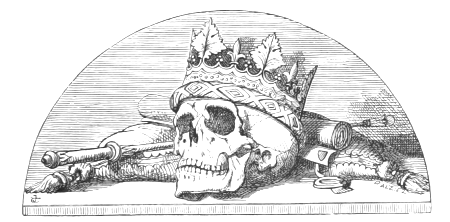
\includegraphics[keepaspectratio=true,scale=.45]{game/SkullLine}

\cbreak

  \mysubsection{Diseased}{effect-diseased}

  The section on \mylink{Diseases}{vulgate-medicine-diseases} is detailed in the \mylink{Vulgate of Medicine}{vulgate-medicine}. Just before the end of each Session, anyone who has come Close to the infected must \RSTRY{\VIG}; if they fail, they become infected with the disease as well.

 \mybold{Effect on Monsters:} Arbiter's discretion.

  \mysubsection{Disgusted}{effect-disgusted}

  You fight through your feelings of revulsion or horror, but all \RO and \RB tries have a -4 modifier as long as you are in the presence of the object of your disgust.

  \mybold{Effect on Monsters:} As long as the Monster is in the presence of the object of its disgust, Attack and Guard tries against the Monster are made at +4.

  \mysubsection{Disarmed}{effect-disarmed}

  Can only affect things held in one hand (like 1h weapons). The item is ripped from your grasp and falls to the ground.  It will take an Action to recover it.

  \mysubsection{Drunk}{effect-drunk}
  
  You take a -1 on any and all \RO and \RB tries, depending on how Drunk you are (you'll see this written as \mybold{Drunk -1}).  You can continue drinking if you desire, taking a cumulative -1 each time, until you reach \mybold{Drunk -4}. Continuing to drink after that point can result in an \mylink{Overdose}{gear-narcotics-overdose}.  The only guaranteed cure is to sleep it off (take a \mylink{Bivouac}{combat-resting-bivouac}).  At the end of your Bivouac, make a \RSTRY{\VIG} - Fallout means you are \mylink{Hung Over}{effect-hung-over}. See the section on \mylink{Narcotics}{gear-narcotics} for more info. 

  \mybold{Effect on Monsters:}  Arbiter's Discretion.

  \mysubsection{Enflamed}{effect-enflamed}

  Dear sweet God, you're on fire! You take d4 damage at the Top of the Moment. The damage die moves \DCUP every Moment afterwards (d6, d8, etc). Damage from the fire bypasses Grit but can be blocked by Armor.

You can douse the flames by spending an entire Moment (2 Actions) performing "stop, drop, and roll".  This can be shortened to a single Action if someone helps you douse the flames. While you're rolling around on the ground, you're \mylink{Prone}{effect-prone}.


  \mysubsection{Enraged}{effect-enraged}

  You immediately attack the closest Monster, dealing +2 damage whenever you strike. You cannot become \mylink{Afraid}{effect-afraid} while you are Enraged, and you cannot do anything defensive, curative, tactical, or cooperate with your Allies. Spellcasting is impossible. If the closest Monster isn't a living thing (a trap or what-have-you), you will attempt to destroy it as quickly and directly as possible. You cannot stop fighting until all the Monsters are dead or have fled (further than Far-Away).  If an Ally hurts you (accidentally or otherwise) during your rage, they are considered a Monster.

  \mybold{Effect on Monsters:}   The Monster gains the \mylink{Rage}{monster-action-rage} Combat Action.

  \mysubsection{Hung Over}{effect-hung-over}

  Roll a d4.  1) You are at -4 on all \RO and \RB tries;  2) You are \mylink{Sickened}{effect-sickened};  3) You are \mylink{Concussed}{effect-concussed}; 4) You are \mylink{Woozy}{effect-woozy}.  The effect lasts until it is removed by Leechcraft, removed with an appropriate tonic (Chymistry) or narcotic, you Bivouac, or you take a number of points of \mylink{Drunk}{effect-drunk} equal to or greater than the number on the die.

  \mybold{Effect on Monsters:}   Arbiter's discretion.

\cbreak

\myimage{game/Horrors}

  \mysubsection{Invisible}{effect-invisible}

  You cannot be seen as long as you don't move.  If you're invisible, you can see other invisible objects.

  \mysubsection{Knocked Out}{effect-knocked-out}

  You immediately drop \mylink{Prone}{effect-prone} and drop any items you're holding.  You cannot Guard, and attacks against you hit automatically, bypass Grit, do maximum damage (Crit), and can only be blocked by Armor.  If the effect does not have a Duration Die associated with it, make an \RSTRY{\VIG} at the top of each Moment; if you succeed, you awaken (but you are still Prone).  Once you awaken, the effect ends.

  \mybold{Effect on Monsters:}   The Monster drops Prone and drops anything it's holding.  Attack tries hit automatically (but don't bypass Soak). If the effect does not have a Duration Die associated with it, make an \RSTRY{\VIG} at the top of each Moment; if it succeeds, the Monster awakens but is still Prone.  



  \mysubsection{Overdosed}{effect-overdosed}

  See more info on \mylink{Overdose}{gear-narcotics-overdose} in the section on \mylink{Narcotics}{gear-narcotics} under \mylink{Gear}{gear}.




  \mysubsection{Paralyzed}{effect-paralyzed}

  You immediately grow rigid - you cannot move or act, even to defend yourself.  Guard tries automatically fail: the attack bypasses Grit, does maximum damage (Crit) and can only be blocked by Armor.  

  \mybold{Effect on Monsters:}   The Monster grows rigid and cannot move or act to defend itself.  Attack tries hit automatically: the attack does maximum damage (Crit) and can only be blocked by Armor.

  \mysubsection{Prone}{effect-prone}

  If you are knocked Prone you must spend an Action getting to your feet.  While you are in a prone position you can continue to Attack and Guard at a -4 penalty.
  
   \mybold{Effect on Monsters:} The Monster must spend an Action getting to its feet (a Basic Maneuver).  The Monster can still attack you and defend itself while it's prone, but your Attack and Guard tries are made at +4.

  \mysubsection{Shaken}{effect-shaken}

  Synonymous with Disgusted, but usually occurs from something that terrifies you.

  \mybold{Effect on Monsters:} Same as Disgusted above.

  \mysubsection{Shocked}{effect-shocked}

  Immediately drop anything you're holding.  If you are shocked as the result of a Horror you have witnessed, your hair turns snow white.

  \mybold{Effect on Monsters:}   The Monster drops whatever it's holding.


  \mysubsection{Sickened}{effect-sickened}

  You are overcome with nausea and begin vomiting, dry-heaving, etc.  You cannot Attack and can only Guard at a -4.

  \mybold{Effect on Monsters:}   The Monster cannot attack, and Attack rolls against the Monster are made at a +4.

\newpage

  \mysubsection{Slept}{effect-slept}

  You are asleep.  Treat yourself as \mylink{Prone}{effect-prone}.  Attacks against you automatically succeed and do maximum damage, which can only be blocked by Armor (taking damage immediately wakes you up).  You can also be awoken with a good, hard slap; bucket of cold water; etc.

    \mybold{Effect on Monsters:}   The Monster is sleeping.  Any damage will wake it up immediately, but Attack tries hit automatically and deal maximum damage (Crit), and will only be blocked by Soak.

  \mysubsection{Stunned}{effect-stunned}

  You are overwhelmed and can only take a Guard Action until the effect ends.

  \mybold{Effect on Monsters:}   The Monster cannot attack.

  \mysubsection{Surprised}{effect-surprised}

  You are surprised and it takes a moment to get your bearings. If Surprise happens as part of an attack, your opponent has \mylink{the Drop}{combat-drop} on you (you can read more about \mylink{the Drop}{combat-drop} in the \mylink{Fighting}{combat-fighting} section of \mylink{Combat}{combat}). Examples of surprise might be: setting off a trap; someone kicking down the door and bum rushing you; a vampire fading in behind you and biting you in the neck; etc. 

  \mybold{Effect on Monsters:}  You have \mylink{the Drop}{combat-drop} on the Monsters!

\cbreak

  \mysubsection{Unhallowed}{effect-unhallowed}
  
  Unhallowed creatures have no soul and exist outside of \mylink{the Dream}{the-dream}. Unhallowed creatures may be harmed by the \mylink{Vulgate of Sacraments}{vulgate-sacraments} and cannot enter \mylink{Hallowed Ground}{miracle-hallowed-ground}.


  \mysubsection{The Vapors}{effect-the-vapors}

  You immediately pass out. Same as \mylink{Slept}{effect-slept} above, but more comical.

    \mybold{Effect on Monsters:}   The Monster passes out; see \mylink{Slept}{effect-slept} above.

  \mysubsection{Woozy}{effect-woozy}

  You take a -4 penalty to \myital{every} \RO and \RB attempt (including Attack and Guard).

  \mybold{Effect on Monsters:} Attack and Guard tries against the Monster are made at a +4.

\myimage{game/Illness}

